\chapter{Structure du site}
\section{MPAs \textit{versus} SPAs \cite{ArchitectureWebApp}}
Traditionnellement, les sites webs \'etaient constitu\'es d'un ensemble de pages diff\'erentes stock\'es sur le serveur et qui seront transmis aux visiteurs suivant au demande. Cette fa\c{c}on de faire est toujours utilis\'e aujourdh'ui puisqu'il a ses avantages. Toutefois, il existe aussi la possibilit\'e de cr\'eer des sites Webs avec une seule page. 


\subsection{Pages Web traditionnels - MPAs (Multi-Page Applications)}
Les applications Web multi-pages impliquent peu de comportement c\^ot\'e client, mais s'appuient plut\^ot sur le serveur pour toutes les navigations, requ\^etes et mises \`a jour que l'application pouvait avoir besoin d'effectuer. Chaque nouvelle op\'eration effectu\'ee par l'utilisateur serait traduite en une nouvelle requ\^ete web, avec pour r\'esultat un rechargement complet de la page dans le navigateur de l'utilisateur. \\

Amazon et Google Docs sont des exemples de telles pages.

\subsection{Applications Web \`a page Unique - SPAs (Single-Page Applications)}
Une application \texttt{Web} \`a page unique (SPA) fonctionne dans un navigateur Web et ne charge qu'une seule page. Il n'a pas besoin de recharger la page pendant son utilisation, surtout que la plupart de son contenu reste le m\^eme, par cons\'equent, seule une partie doit \^etre mise \`a jour. Lorsque le contenu doit \^etre mis \`a jour, le SPA le fait via des APIs.\\
De cette façon, les utilisateurs peuvent consulter un site Web sans charger l'int\'egralit\'e de la nouvelle page ni les donn\'ees du serveur. En cons\'equence, les performances augmentent et vous avez l'impression d'utiliser une application native. Il offre une exp\'erience Web plus dynamique aux utilisateurs. \\

Gmail, Facebook, Trello et Google Maps sont tous des applications \`a page unique qui offrent une exp\'erience utilisateur exceptionnelle dans le navigateur sans rechargement de page.


\subsection{Diff\'erences}
Les SPAS ont un temps de chargement plus longue, mais offrent des performances plus rapides et une navigation fluide apr\`es le chargement. Les MPAs peuvent \^etre relativement lents et n\'ecessitent une connexion Internet de premier ordre, notamment en ce qui concerne les \'el\'ements graphiques.\\

Les MPAs sont efficaces lorsque :
\begin{itemize}
	\item[-] Les exigences c\^ot\'e client de l'application sont simples, voire en lecture seule.
	\item[-] L'application fonctionne dans les navigateurs sans prise en charge de JavaScript.
	\item[-] L'application est destin\'ee au public et b\'en\'eficie de la d\'ecouverte et des r\'ef\'erences des moteurs de recherche.
\end{itemize}

Les SPAs sont efficaces lorsque :
\begin{itemize}
	\item[-] L'application pr\'esente une interface utilisateur riche avec de nombreuses fonctionnalit\'es.
	\item[-] L'\'equipe est familiaris\'ee avec le d\'eveloppement JavaScript, TypeScript ou Blazor WebAssembly.
	\item[-] L'application expose une API pour d'autres clients (internes ou publics).
\end{itemize}

\vspace{1cm}

\begin{table}[!ht]
	\centering
	\begin{tabular}{ | a || m{0.2\textwidth}  m{0.2\textwidth}|}
		%					\hline
		\rowcolor{lightgray}
		{\Large \textsc{Facteurs}} & \textbf{MPA} & \textbf{SPA}\\
		\hline
		\hline
		\textbf{Familiarit\'e de l'\'equipe avec JavaScript ou TypeScript} & Minimale & Requise\\
		\hline
		\textbf{Gestion du navigateur sans script} & Prise en charge & Non prise en charge \\
		\hline
		\textbf{Comportement minimal des applications c\^ot\'e client} &	Bien adapt\'e & Bien adapt\'e \\
		\hline
		\textbf{Interface utilisateur riche et complexe} &	Limit\'e & Bien adapt\'e \\
		\hline
		\textbf{D\'eveloppement} & Simple & Complexe\\
		\hline
		\textbf{Visibilit\'e sur les moteurs de recherche} & \'Elev\'ee & Faible \\
		\hline
		\textbf{Changement par un non-d\'eveloppeur} & Prise en charge & Non prise en charge\\
		\hline
	\end{tabular}
	\caption{Tableau r\'ecapitulatif - Principales crit\`eres de choix entre MPAs et SPAs}
	\label{tableChoixEntreMPAetSPA}
\end{table}

\paragraph{} Pour garantir un excellent service aux utilisateurs du logiciel, g\'erer les divers fonctionnalit\'es requises pour notre syst\`eme sans erreur, nous avons opt\'e pour le mod\`ele SPA (Single Page Application). Nous devrons donc trouver un moyen pour augmenter la visiblit\'e du site sur les moteurs de recherche et  d\'evelopper un outils de gestion du logiciel pour r\'epondre aux exigences du projet (Voir Sections~\ref{SectQualiteDuSysteme} et~\ref{SectionBesoinsFonctionnels}).



\subsubsection{Fonctionnement du mod\`ele SPA}

\begin{figure}[!ht]
	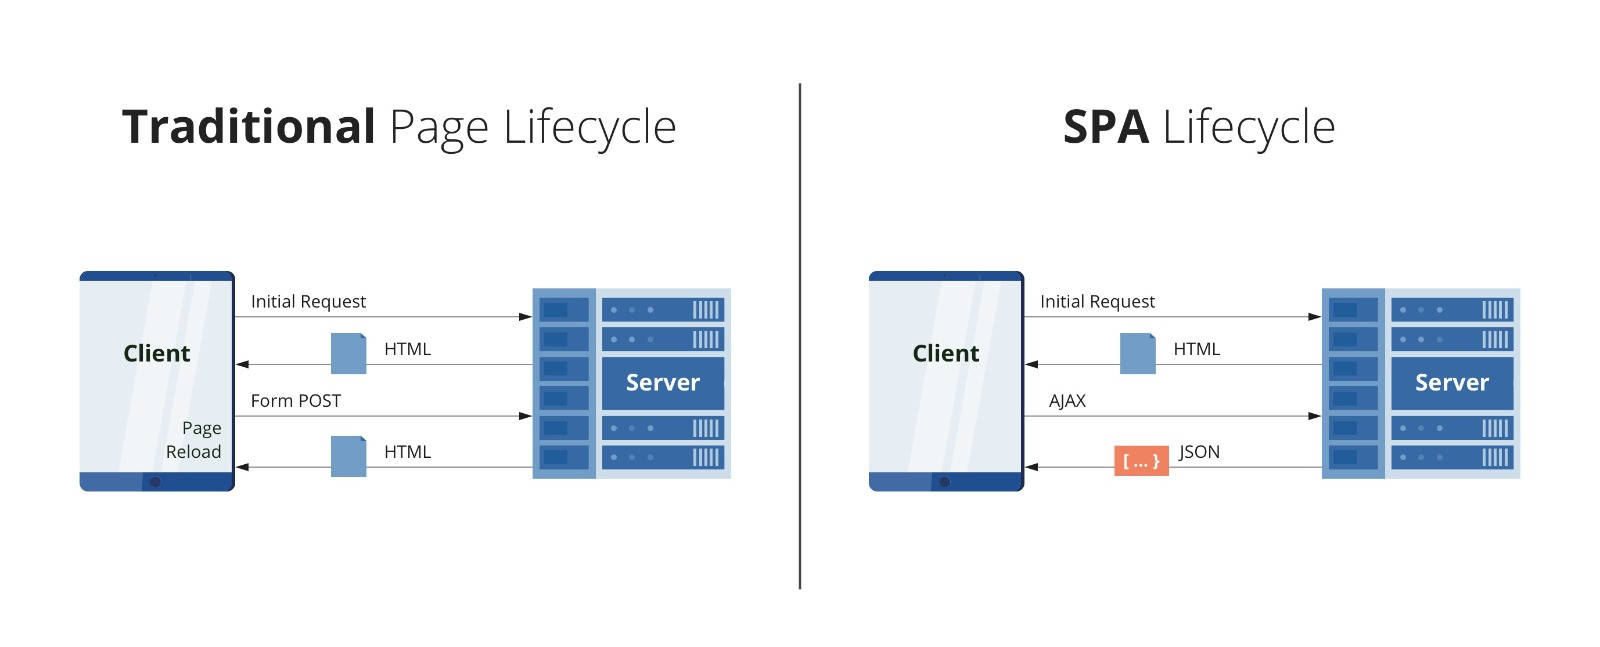
\includegraphics[width=0.7\linewidth]{Pictures/SPALifeCycle.jpg}
	\centering
	\caption{Cycle de vie d'un SPA par rapport \`a celui d'un MPA\cite{CycleDeVieMPAvsSPA}}
	\label{FigSPA}
\end{figure}


Le mod\`ele SPA repose sur les principes suivants :
\begin{enumerate}
	\item Le SPA utilise principalement des technologies de rendu c\^ot\'e client, comme JavaScript, TypeScript et autres pour g\'erer la logique de l'interface utilisateur et communiquer avec le serveur via des API web.
	\item Le SPA charge initialement le code HTML, CSS et JavaScript n\'ecessaire pour afficher la page web. Ensuite, il ne charge que les donn\'ees n\'ecessaires pour mettre \`a jour le contenu de la page, en utilisant des formats l\'egers comme JSON ou XML.
	\item Le SPA utilise le concept de routage c\^ot\'e client, qui consiste \`a modifier l'URL de la page sans recharger la page, en utilisant \texttt{l'API History} du navigateur. Ainsi, le SPA peut offrir une navigation fluide et intuitive, tout en conservant la possibilit\'e d'utiliser les boutons Pr\'ec\'edent et suivant du navigateur.
	\item Le SPA offre une exp\'erience utilisateur plus rapide, plus r\'eactive et plus proche d'une application native, car il \'evite les temps de chargement et les rafraîchissements de la page. Il peut \'egalement fonctionner hors ligne, en utilisant des technologies comme le \texttt{Service Worker} ou le \texttt{Local Storage}.
\end{enumerate}


\section{Architecture du syst\`eme\cite{Architecture3Niveau}}
\label{ChapArchitectureDuSysteme}
L'architecture d'un syst\`eme est la mani\`ere de concevoir et d'organiser les diff\'erents \'el\'ements qui le composent. Il s'agit d'une repr\'esentation abstraite d'un syst\`eme exprim\'ee essentiellement \`a l'aide des composants du logiciels et de leurs interactions. L'architecture d'un syst\`eme permet de d\'efinir la structure, le comportement, la qualit\'e et les contraintes du syst\`eme, en fonction des besoins et des objectifs du projet. Elle facilite par cons\'equent la conception, le d\'eveloppement, le d\'eploiement et la maintenance de celui ci. Il existe plusieurs architecture possible pour une application web dont: l'architecture monolithique, les architectures \`a  N-niveaux, Architecture hexagonal (Aussi appel\'e Architecture Port-et-adapter)  \\

\subsection{Architecture de \projectName}
L'architecture adopt\'ee pour notre syst\`eme est l'architecture \`a trois niveaux (appel\'ee architecture \texttt{3-tiers}) client/application/ressource (Voir Figures~\ref{FigArchitecture} et~\ref{FigArchitecture1}).  Le principal avantage de l'architecture \`a trois niveaux r\'eside dans la s\'eparation logique et physique des fonctionnalit\'es. Chaque niveau peut fonctionner sur un syst\`eme d'exploitation et une plate-forme de serveur distincts (par exemple : un serveur Web, un serveur d'applications, un serveur de base de donn\'ees).\\
Outre cet avantage essentiel, elle offre une plus grande flexibilit\'e du fait qu'un \'el\'ement peut \^etre remplac\'e sans devoir changer toute l'architecture, une s\'ecurit\'e peut \^etre impl\'ement\'ee \'e chaque service et \`a chaque niveau. Et enfin, puisque les t\^aches sont partag\'ees elle offre de meilleures performances surtout une fiabilit\'e am\'elior\'ee. Elle est aussi r\'esistante aux pannes puisqu'une panne dans un niveau est moins susceptible d'avoir un impact sur la disponibilit\'e ou les performances des autres niveaux.

	\begin{figure}[ht]
		\centering
		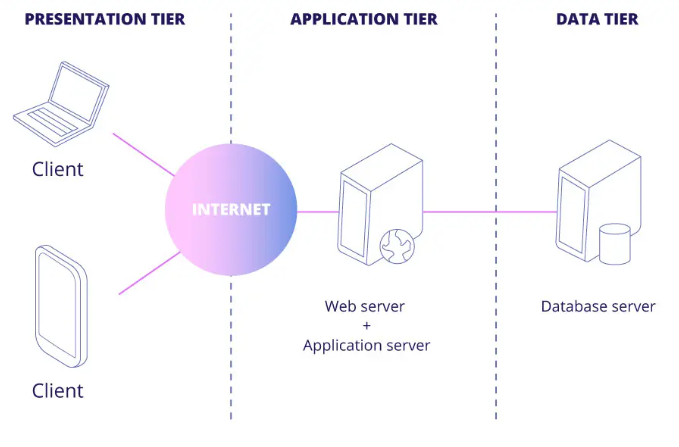
\includegraphics[width=0.5\textwidth]{Pictures/SystemStruct.png}
		\caption{Architecture physique \`a trois niveaux\cite{SourceFigArchitecture}}
		\label{FigArchitecture}
	\end{figure} 


L'architecture \`a trois niveaux organise les applications en trois niveaux informatiques logiques et physiques : le niveau de pr\'esentation, ou interface utilisateur ; le niveau application, o\`u les donn\'ees sont trait\'ees ; et le niveau des donn\'ees, o\`u  les donn\'ees associ\'ees \`a l'application sont stock\'ees et g\'er\'ees.
\subsubsection{Partie cliente - Front-End}
Cette partie est constitu\'ee des nœuds et elle consiste aussi \`a la r\'ealisation des diff\'erentes interfaces de l'application et leur affichage. En gros ce sont les demandeurs de ressources.

\subsubsection{Partie serveur (serveur d'application)}
Permet de r\'epondre de mani\`ere automatique \`a des demandes envoy\'ees par la partie cliente. C'est elle qui se charge de fournir la ressource tout en faisant appel \` un autre serveur (serveur base de donn\'ees).

\subsubsection{Partie serveur base de donn\'ees}
Permet l'insertion, la consultation des donn\'ees et la mise \`a jour du syst\`eme. Elle fournit un service au serveur d'application.

